\documentclass{beamer}
\usetheme{CambridgeUS}
\usecolortheme{seagull}
\usepackage{comment}
\usepackage{bibunits}  
\usepackage{xmpmulti}
\usepackage{animate}

\definecolor{beamer@blockbg}{rgb}{0.7,0.1,0.1}
\title[cde-Rkeras-intro]{An introduction to conditional density estimation using the R interface to Keras
}
\titlegraphic{\centering\vspace{-0.5cm}
\includegraphics[width=0.35\linewidth]{{Images/Kaust-Logo.png}}}
\author[Jordan Richards]{Jordan Richards}
\institute[KAUST]{King Abdullah University of Science and Technology (KAUST)}
\date{\today}
\usepackage{colortbl}
\usepackage[T1]{fontenc}
\usepackage{lmodern}
\definecolor{bostonuniversityred}{rgb}{0.8, 0.0, 0.0}
\definecolor{vermilion}{rgb}{0.9, 0.26, 0.2}
\bibliographystyle{apalike}

\usepackage{siunitx}

\setbeamercovered{transparent}

\begin{document}
\maketitle
\begin{frame}{Outline}
\tableofcontents
\end{frame}
\section{Background}
\begin{frame}{What is Keras?}
\begin{itemize}
\item Keras is a \textbf{high-level API} for fast deep learning developed by \textbf{Google} and written primarily in \textbf{Python}, released in 2015
\item Whilst it used to support a number of different \textbf{back-ends} (Theano, MILA; CNTK, Microsoft) it now solely runs on top of \textbf{Tensorflow}
\item Tensorflow is a free open-source machine learning (not just DL) library written in Python, C++ and CUDA (for \textbf{GPUs}) that does all of the lower-level computations for Keras
\item Keras is the \textbf{most popularly applied deep learning software} due to its simple yet powerful framework, followed closely by Facebook's PyTorch. This can also be used in R (see \url{https://www.rstudio.com/blog/torch/})
\end{itemize}

\end{frame}
\begin{frame}{What is (parametric) conditional density estimation?}
Let's say you have a \textbf{response} variable $Y$ with \textbf{covariates/predictors} $\mathbf{X}$:
\begin{itemize}
\item Conditional density estimation is a \textbf{generalisation} of normal (mean/least-squares) regression
\item In mean regression, we model $\mathbb{E}[Y|\mathbf{X}]$ as a function $m$ of predictors. For CDF, we model the \textbf{entire conditional density} $f(Y|\mathbf{X})$
\item In a \textbf{parametric framework}, we let $Y|\mathbf{X}\sim \mathcal{F}(\boldsymbol{\theta})$ for a parameter set $\boldsymbol{\theta}$ and then let $\boldsymbol{\theta}$ be a function $m$ of observations $\mathbf{x}$ of $\mathbf{X}$
\item Prediction $\Leftrightarrow$ Gaussian density estimation (with fixed $\sigma=1$). Classification problems $\Leftrightarrow$ Multinomial density estimation
\item We are going to estimate $m(\mathbf{x})$ using \textbf{Deep Learning}
\end{itemize}
\end{frame}

\begin{frame}{Objectives}
The objectives of this short-course are:
\begin{itemize}
\item Understand the basics of deep learning and neural networks
\item Build and train simple feed-forward prediction and regression models using the R interface to Keras
\item Perform conditional density estimation using neural networks
\end{itemize}
\end{frame}

\begin{frame}{Some suggested reading}
For deep learning:
\begin{itemize}
\item Chollet, F. with Allaire, J. J. (2018). Deep learning with R 
\item Any of the multitude of Keras for R blogs, see e.g., \href{https://blogs.rstudio.com/ai/posts/2019-11-27-gettingstarted-2020/}{blogs.rstudio.com}, \href{https://www.r-bloggers.com/2021/12/using-keras-for-deep-learning-with-r/}{r-bloggers.com}, \href{https://towardsdatascience.com/r-vs-python-image-classification-with-keras-1fa99a8fef9b}{towardsdatascience}, \href{https://www.analyticsvidhya.com/blog/2017/06/getting-started-with-deep-learning-using-keras-in-r/}{analaticsvidyha}. (Even those that give code written in Python as it's very easy to translate!)
\item Rodrigeus, F., Pereira, F. C., (2022). Beyond expectation: Deep joint mean and quantile regression for spatiotemporal problems (Nice introduction to CNNLSTMs for quantile regression)
\item There's some really good \url{https://www.coursera.org/}{coursera} courses for deep learning, particularly with Python
\end{itemize}
\end{frame}

\begin{frame}{Some suggested reading}
For CDE (tailored towards extremes):
\begin{itemize}
\item Cannon, A. J. (2010). A flexible nonlinear modelling framework for nonstationary generalized extreme value analysis in hydroclimatology 
\item Cannon, A. J. (2011). GEVcdn R package
\item  Carreau, J., Bengio, Y. (2007). A hybrid Pareto model for asymmetric fat-tailed data
\item Richards, J., Huser, R., (2022). High-dimensional extreme quantile regression using partially-interpretable neural networks: With application to U.S. wildfires
\end{itemize}
\end{frame}

\section{Installing the R interface to Keras}
\begin{frame}{Installation}
 First thing's first, let's get Keras installed
\begin{itemize}
\item Open \textit{installation.R}
\item Download and install Python 3.8.4 from \url{https://www.python.org/downloads/macos/} (unless you already have a working version of Python $\geq 3.5$)
\item Install the \texttt{keras} and \texttt{tensorflow} R packages
\item Create a virtual Python environment 
\item Configure the Rstudio Python interpreter (you will need to restart the R session for this)
\item Install the latest versions of the Python libraries \textit{tensorflow} and \textit{keras}
\end{itemize}
\textcolor{red}{Don't touch any Python2 installations!}
\end{frame}
\begin{frame}
\begin{center}
\Huge Deep learning
\end{center}
\end{frame}
\section{Deep learning}
\begin{frame}{What is deep learning?\footnote{Copyright belongs to \url{https://flatironschool.com/blog/deep-learning-vs-machine-learning/}}}
\begin{figure}
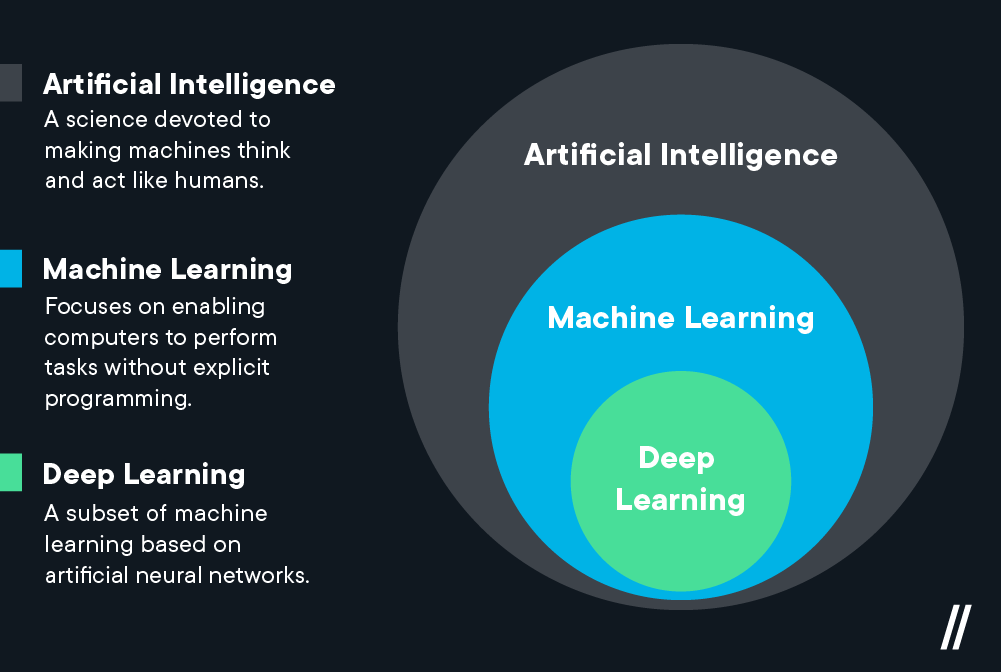
\includegraphics[width=0.75\linewidth]{Images/AI.png}
\end{figure}
\end{frame}
\begin{frame}{Deep learning vs. machine learning\footnote{Copyright belongs to \url{https://levity.ai/blog/difference-machine-learning-deep-learning}}}
\begin{itemize}
\item Specifically uses \textbf{artificial neural networks} (ANNs)
\item Algorithms are much \textbf{more complex} and require \textbf{less human intervention} $\Rightarrow$ no manual feature extraction/engineering required
\item Typically requires \textcolor{red}{substantially more data} to train. Gives rise to the concept of \textbf{transfer learning}, i.e., using pre-trained models 
\end{itemize}
\begin{figure}
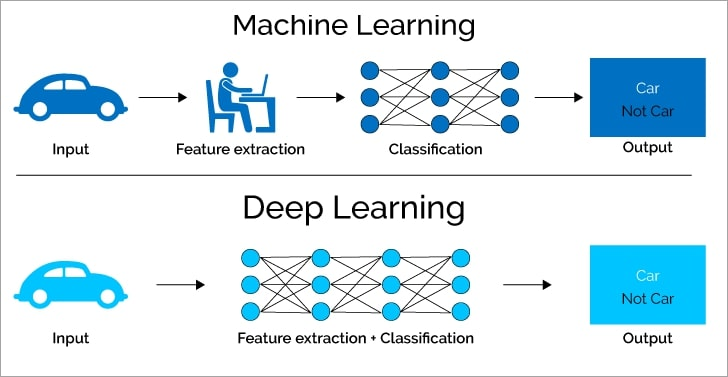
\includegraphics[width=0.5\linewidth]{Images/ML.jpeg}
\end{figure}
\end{frame}
\subsection{Basics of neural networks}

\begin{frame}{Basics of neural networks}
\begin{minipage}{0.70\linewidth}
\begin{itemize}
\item A neural network is an algorithm designed to mimic the \textbf{human brain}.
\item It can be constructed as a \textbf{directed graph} with a single input and a single output, with a dense network of \textbf{interconnected nodes} in-between
\item Data is input into the graph and information is extracted at each node, a.k.a \textbf{perceptron}. An output is provided at the end of the network.
\item Similarly brain activity occurs when a stimuli enters the system, information is based through the network via \textbf{neurons} that extra relevant information and this information passes to some area of the brain that forces a response (output)
\end{itemize}
\end{minipage}
\begin{minipage}{0.29\linewidth}
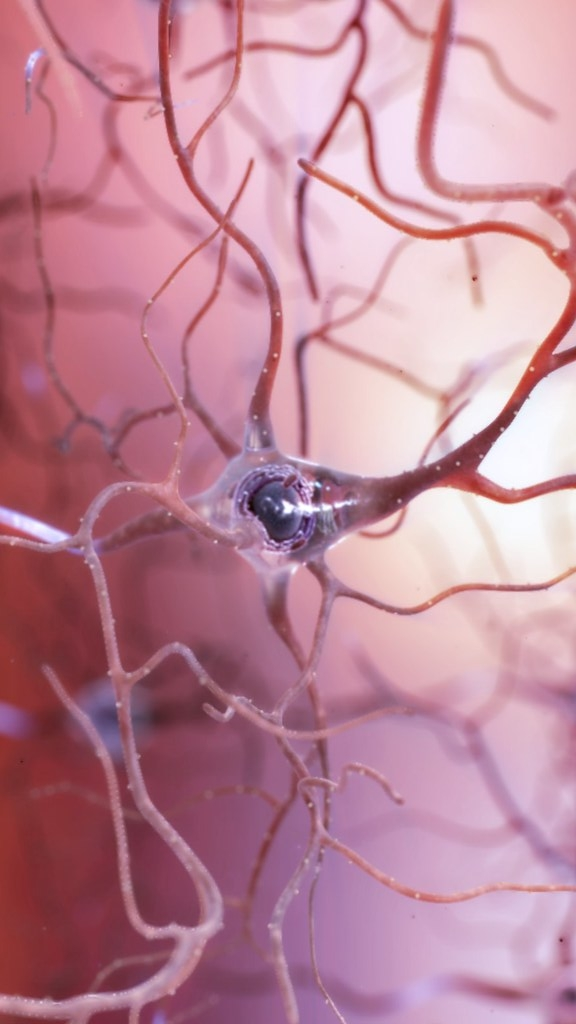
\includegraphics[width=0.9\textwidth]{Images/neuron.jpg}
\end{minipage}
\end{frame}
\begin{frame}
 Nodes in a neural network are arranged in layers:
\begin{itemize}
\item A single node may be connected to several nodes in the layer above, from which it \textbf{receives information}, and to the layer below, which it \textbf{feeds information}
\item Most neural networks are \textbf{``feed forward"} - information is passed forward, layer-to-layer, in one direction only
\item Different information is extracted at each layer in a \textbf{hierarchical} fashion, i.e., the most important aspects first
\item The ``deep" in deep learning refers to the depth of layers in a neural network as well as its hierarchical nature
\end{itemize}
\end{frame}
\subsection{Architecture}
\begin{frame}
\begin{center}
\Huge Architecture
\end{center}
\end{frame}
\begin{frame}{Typical structure\footnote{Copyright belongs to \url{https://www.ibm.com/cloud/blog/ai-vs-machine-learning-vs-deep-learning-vs-neural-networks}}}
\begin{figure}
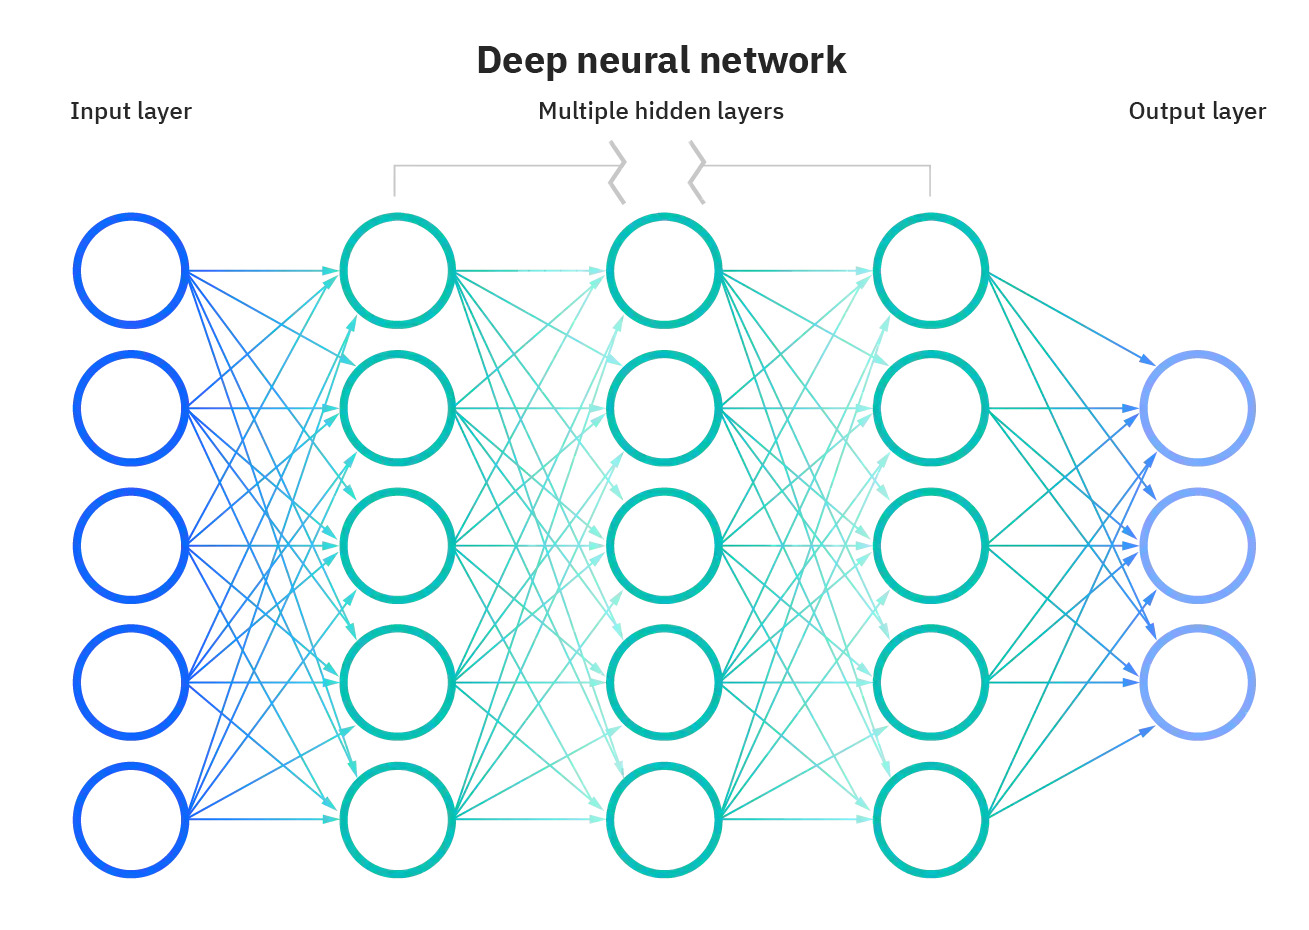
\includegraphics[width=0.7\textwidth]{Images/nn.jpg}
\end{figure}
\end{frame}
\begin{frame}{Typical structure}
\begin{itemize}
\item A \textbf{single input layer}. Each input would be a single predictor variable in the form of a scalar value, a sequence or an image (or even a sequence of images!).
\item \textbf{A single output layer}. For prediction or classification problems, we would have a single node here. For CDE, we would have $|\boldsymbol{\theta}|$ nodes.
\item A collection of \textbf{hidden layers}. Preferably more than one! In the previous example, each hidden layer has a \textbf{width} of five.
\item Calculations are completed at each node in the hidden layer. These are parameterised by \textbf{weights and biases}.
\item The calculations within a layer are of a certain ``type". We will consider standard, convolution and recurrent layers.
\end{itemize}
We refer to the structure of a neural network as its \textbf{architecture}.
\end{frame}

\begin{frame}{Standard ``vanilla" MLPs}
A standard multi-layered perception uses $\texttt{layer\_dense}$ in $\texttt{Keras}$ and takes in a vector of values, i.e., a scalar for each input node. Let's say that $\mathbf{x}\in\mathbb{R}^d$ is our input - so the previous layer had $d$ outputs! We take some
\begin{itemize}
\item Weights: $w_i \in \mathbb{R}$ for $i=1,\dots,d$
\item Bias: $b\in\mathbb{R}$ 
\item Calculate $\sum^d_{i=1}w_ix_i + b$
\item And apply an \textbf{activation function} $a$ to get:
\end{itemize}
\[a\left(\sum^d_{i=1}w_ix_i + b\right).\]
And that's it!
\end{frame}
\begin{frame}
\begin{figure}
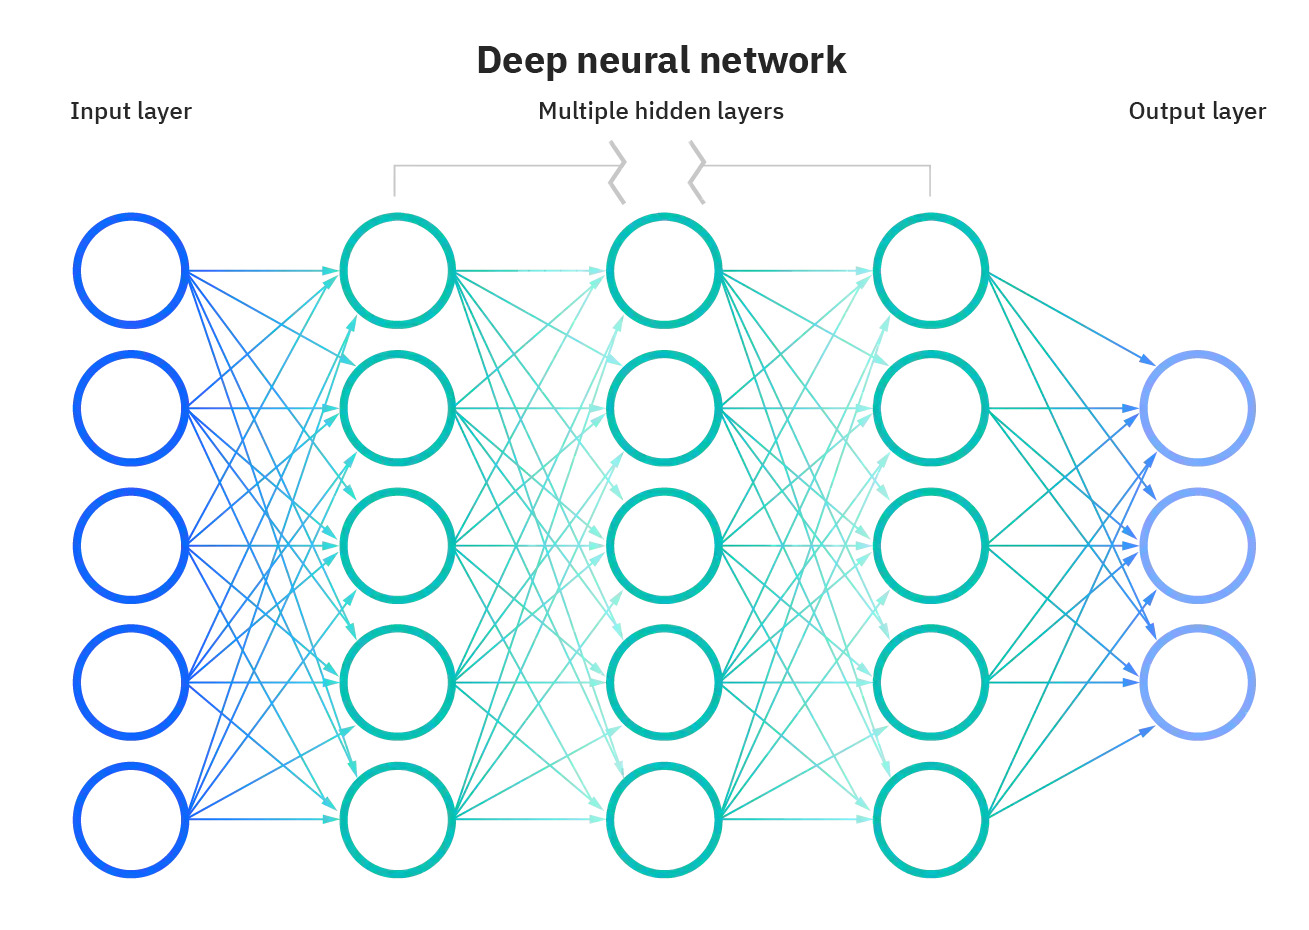
\includegraphics[width=0.7\textwidth]{Images/nn.jpg}
\end{figure}
\end{frame}
\begin{frame}{Activation function\footnote{\url{https://en.wikipedia.org/wiki/Activation_function}}}
The activation function defines the \textbf{output of the node}. There's a range of different functions that you can use (see \url{https://keras.rstudio.com/reference/activation_relu.html}), but typically they must satisfy two properties:  
\begin{itemize}
\item \textbf{Nonlinear}! If all nodes had linear activation, this would just be a linear regression model. A two-layered NN with non-linear activations is a \textbf{universal function approximator}.
\item \textbf{Continuously differentiable}. Needed for gradient-based optimisation.
\end{itemize}
You can think of the activation function as an analogue to the link function in regression. In fact, a single-layered NN is simply a \textbf{generalised linear regression model}. We can think of CDE using NNs as a\textbf{hierarchical generalised linear model}.
\end{frame}
\begin{frame}{ReLu activation}
An activation function that's popularly applied is the \textbf{rectified linear unit}:
\begin{itemize}
\item Older neural networks relied on sigmoid or $\tanh$ activation functions
\item These suffered from the \textit{vanishing gradient problem}\footnote{The networks we will be considering will not be overly deep, so this problem does not occur. For details, see \url{https://machinelearningmastery.com/rectified-linear-activation-function-for-deep-learning-neural-networks/}}, which made it \textcolor{red}{difficult to efficiently train deep networks}
\item The Relu replaced these. It has the form $a(x)=\max\{x,0\}$.
\end{itemize}
\begin{minipage}{0.49\linewidth}
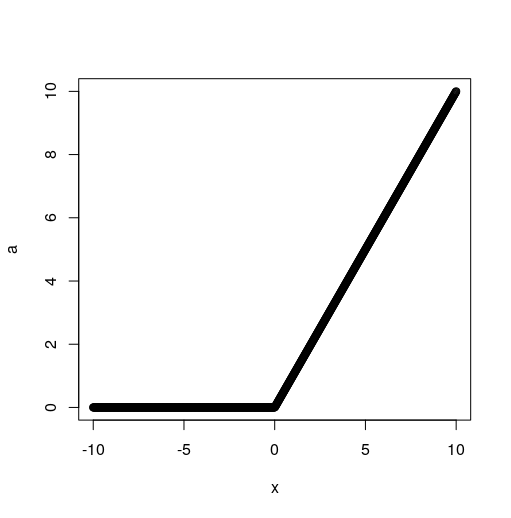
\includegraphics[width=0.5\textwidth]{Images/ReLu.png}
\end{minipage}
\begin{minipage}{0.49\linewidth}
\begin{itemize}
\item The neuron ``activates" only if \textbf{enough information passes through} (think pain receptors)
\item One drawback: \textcolor{red}{not differentiable at zero}
\end{itemize}
\end{minipage}
\end{frame}
\begin{frame}{Convolution layers\footnote{Copyright belongs to \url{https://machinelearningmastery.com/convolutional-layers-for-deep-learning-neural-networks/}}}
A \textbf{convolution layer} acts on an image, not a vector of inputs. The image can be 1D (e.g., text), 2D or 3D (e.g., a video or 3D model)
\begin{minipage}{0.49\linewidth}
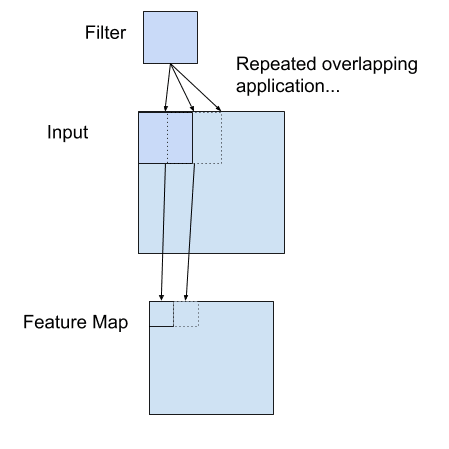
\includegraphics[width=\textwidth]{Images/cfilter.png}
\end{minipage}
\begin{minipage}{0.49\linewidth}
\begin{itemize}
\item A convolution filter/kernel of a certain dimension is passed over the image
\item The filter starts in a corner of the image. A convolution is performed, and then the filter moves one horizontal ``stride". Once it reaches the edge, it moves one vertical stride down. 
\end{itemize}
\end{minipage}
\end{frame}
\begin{frame}{Convolution layers\footnote{Copyright belongs to \url{https://machinelearningmastery.com/convolutional-layers-for-deep-learning-neural-networks/}}}
\begin{minipage}{0.39\linewidth}
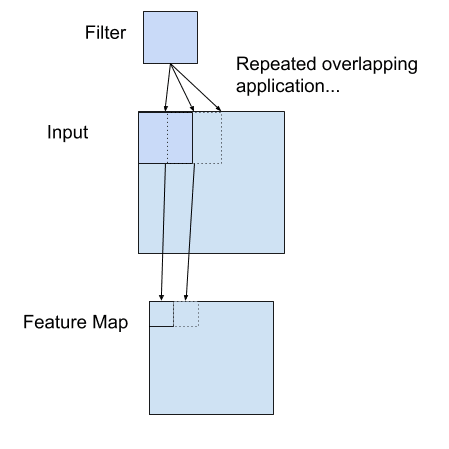
\includegraphics[width=\textwidth]{Images/cfilter.png}
\end{minipage}
\begin{minipage}{0.59\linewidth}
\begin{itemize}
\item After the filter has passed over the entire image, a \textbf{feature map} will be produced. The dimension of the feature map will be determined by the filter dimension and the strides
\item An image can have multiple ``channels", i.e., different colours, inputs, each with its own filter
\item The feature maps for the different channels are added, a bias is introduced and then $a$ is applied 
\item A layer can have \textbf{multiple filters}, similar to nodes in a densely-connected network
\end{itemize}
\end{minipage}
\end{frame}
\begin{frame}{Convolutions}
\begin{itemize}
\item Each filter has an array of weights corresponding to its dimension. A $3\times 4$ filter will have a $3\times 4$ matrix of weights
\item A convolution is simply the \textbf{dot product} of the filter weights and the image values
\item Unless the filter has all dimensions one and a stride of one (\textbf{this is just a dense layer!}), the outputted feature map will have a smaller dimension that the input images. This can be rectified using \textbf{padding}, i.e., adding zeroes to the boundaries of the image
\item \textcolor{green}{Very good for capturing spatial characteristics} in data
\end{itemize}
\end{frame}
\begin{frame}

\end{frame}
\begin{frame}{Recurrent layers\footnote{Copyright belongs to \url{https://www.ibm.com/cloud/learn/recurrent-neural-networks}}}
A recurrent layer takes in as input a sequence of vectors/images. Let's say that the input is the sequence of vectors $\{\mathbf{x}_t:t=1,\dots,T\}$ where $\mathbf{x}_t\in\mathbb{R}^d$ for all $t$.

\begin{figure}
\centering
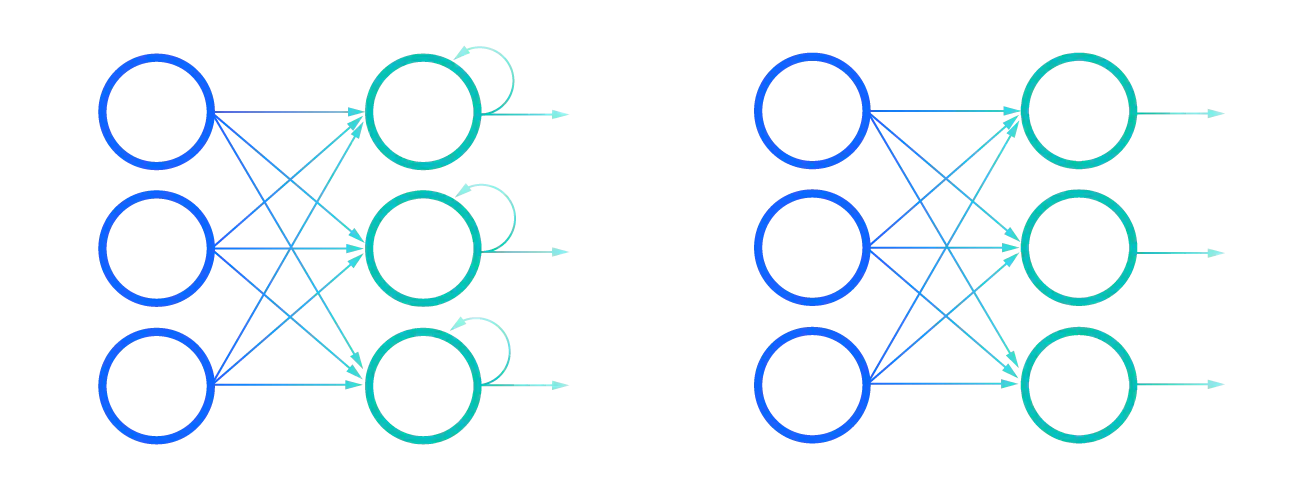
\includegraphics[width=0.7\textwidth]{Images/rnn.png}
\end{figure}
Once an input enters the layer, it becomes stuck in a \textbf{recurrence loop} - the output from the computation using the first input vector $\mathbf{x}_1$ becomes an input for the computation on $\mathbf{x}_2$ (and so on...).
\end{frame}
\begin{frame}{Recurrent layers\footnote{Copyright belongs to \url{https://www.ibm.com/cloud/learn/recurrent-neural-networks}}}
\begin{figure}
\centering
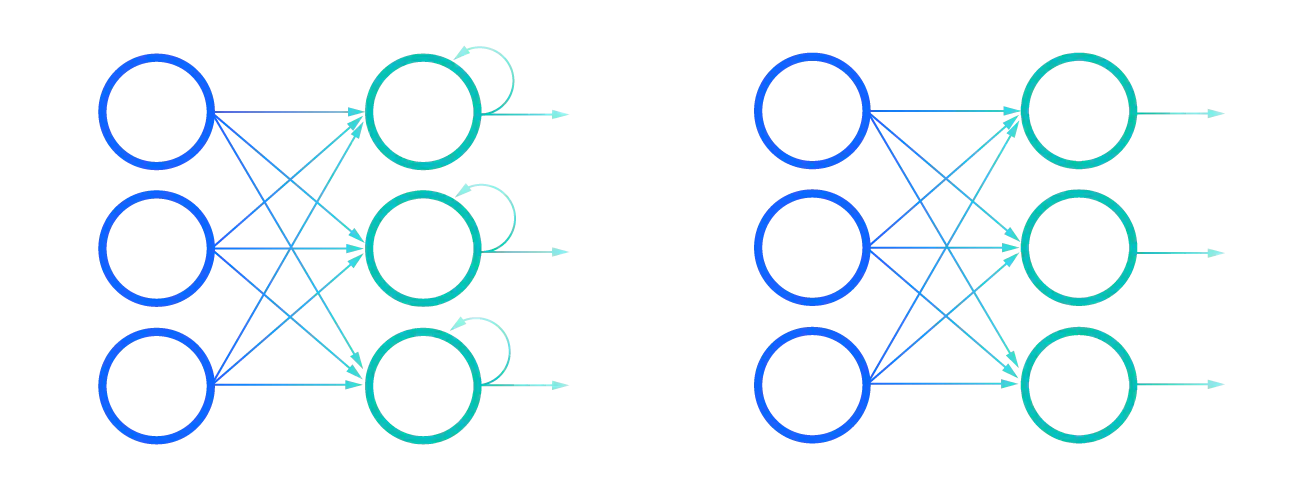
\includegraphics[width=\textwidth]{Images/rnn.png}
\end{figure}

\end{frame}
\begin{frame}{Recurrent layers\footnote{Copyright belongs to \url{https://www.ibm.com/cloud/learn/recurrent-neural-networks}}}
Let's consider a very basic example of a recurrent layer and just look at the computations at a single recurrent node. The output from the first vector in the sequence $\mathbf{x}_1$ is $a(m_1+b)$ where
\[
m_1=\sum^d_{i=1}x_{i,1}w_i.
\]
The output $a(m_1+b)$ moves to the next layer, but the information $m_1$ returns back into the same layer.
\begin{figure}
\centering
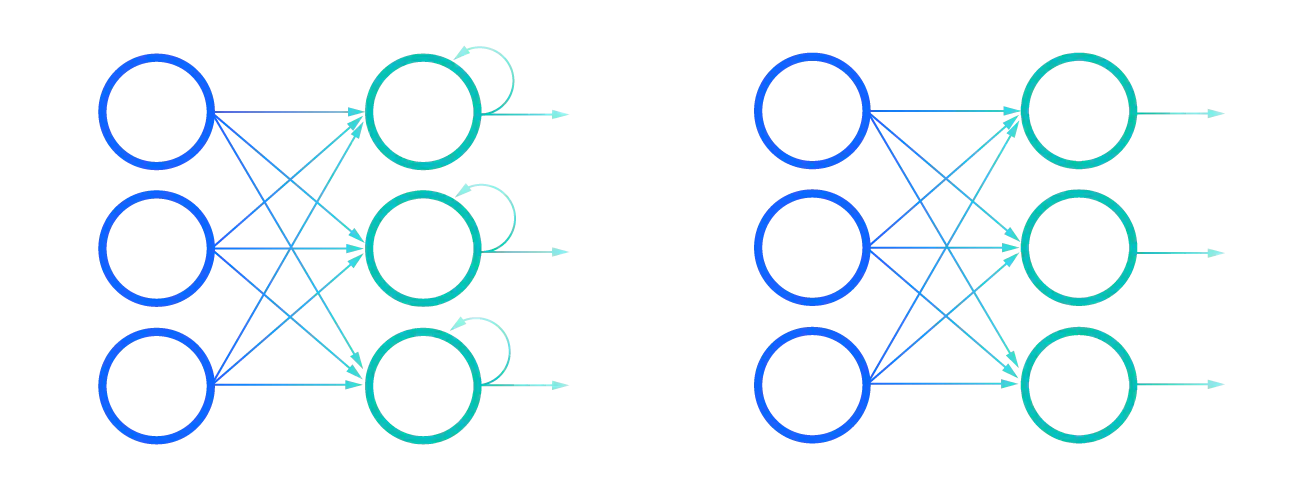
\includegraphics[width=0.5\textwidth]{Images/rnn.png}
\end{figure}
\end{frame}
\begin{frame}{Recurrent layers\footnote{Copyright belongs to \url{https://www.ibm.com/cloud/learn/recurrent-neural-networks}}} The output from the second input $\mathbf{x}_2$ is $a(m_2+b)$ where
\[
m_2=\sum^d_{i=1}x_{2,1}w_i+m_1+b.
\]
So now the output $a(m_2+b)$ contains information from the previous vector in the sequence! And this procedure is repeated for the \textbf{entire sequence} and for all nodes.
\begin{figure}
\centering
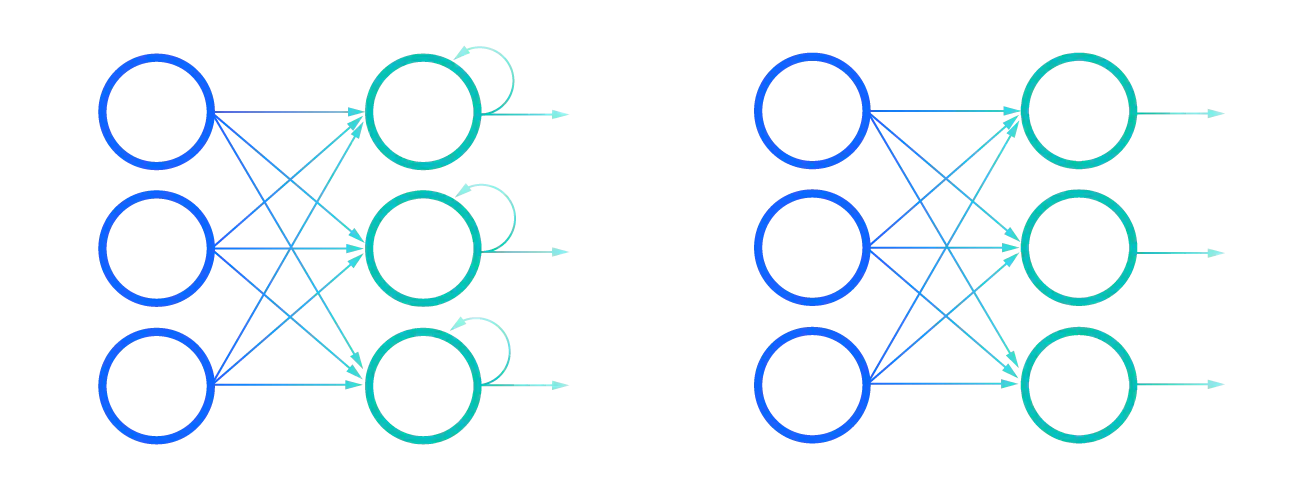
\includegraphics[width=0.5\textwidth]{Images/rnn.png}
\end{figure}
\end{frame}

\begin{frame}{Some points...}
\begin{itemize}
\item These simple layers can be implemented using $\texttt{layer\_simple\_rnn}$
\item Generally these are not used anymore due to numerical stability problems. People now use \textbf{Long Short-Term Memory} layers\footnote{S. Hochreiter; J. Schmidhuber (1997). "Long short-term memory". Neural Computation. 9 (8): 1735–1780.}, implementable by $\texttt{layer\_lstm}$.
\item The intuition is the same, but these layers have ``forget gates" which allow them to forget \textbf{useless information} and avoids numerical instability, i.e., vanishing/exploding gradients
\end{itemize}

\end{frame}
\begin{frame}{Some points...}
\begin{itemize}
\item We considered a dense ``vanilla" recurrent layer. We can have recurrent convolutional layers instead (see e.g., $\texttt{layer\_conv\_lstm\_2d}$), which captures temporal structure within sequences of images
\item The introduction of a recurrent layer means that the NN is no longer ``feed-forward"; unlike like the previous layers, computations for recurrent layers \textcolor{red}{cannot be done in parallel}. This makes training more \textcolor{red}{computationally demanding} and not suitable for laptop-based work. I've not included an explanation of their implementation in $\texttt{Keras}$, but I can provide \textbf{help/code on request}.
\end{itemize}
\end{frame}
\subsection{Training}
\begin{frame}
\begin{center}
\Huge Training
\end{center}
\end{frame}
\begin{frame}{Loss}
Training a neural network, i.e., estimating the weights and biases, is done by optimizing some \textbf{loss function}. Let's say we have $N$ observations of the response $y_1,y_2,\dots$ and the neural network predicts some output $\hat{\mathbf{y}}_1,\hat{\mathbf{y}}_2,\dots$ (could be a vector!). We write the loss function as $l({y},\hat{\mathbf{y}}).$
\end{frame}
\begin{frame}{Loss}
 Whilst the NN architecture can be standard for any task, the loss function must be \textbf{very specific}! Examples include:
\begin{itemize}
\item MSE: $(1/N)\sum^N_{i=1}(y_i-\hat{y}_i)^2$ (mean prediction)
\item MAE: $(1/N)\sum^N_{i=1}|y_i-\hat{y}_i|$ (median prediction)
\item Binary cross-entropy (if $\hat{y}_i\in(0,1)$ and $y_i=0$ or $1$): $-(1/N)\sum^N_{i=1}(y_i\log\hat{y}_i+(1-y_i)\log(1-\hat{y}_i))$. Two-class Classification, but can be extended to more than two classes.
\end{itemize}
For CDE, we will use the negative log-likelihood as the loss function. Here $\hat{\mathbf{y}}$ will be the parameters for distribution we are fitting.
\end{frame}
\begin{frame}{Training}
The loss function is minimised using a form of \textbf{gradient descent}. Neural networks are trained for a \textbf{finite number of epochs} (iterations). Let's say all of the trainable weights and parameters for our NN are contained in some set $\boldsymbol{\Theta}$.   For epoch $i$:
\begin{enumerate}
\item We go forward through the network to compute $\hat{{y}}$ given the current state of the network. This allows us to evaluate $l({y},\hat{\mathbf{y}})$.
\item We move back through the network to compute (exactly) $\nabla l({y},\hat{\mathbf{y}})$ w.r.t $\boldsymbol{\Theta}$.
\item We update the parameters using
\[
\boldsymbol{\Theta}^{(i+1)}=\boldsymbol{\Theta}^{(i)}-\boldsymbol{\lambda}^{(i)}\nabla l({y},\hat{\mathbf{y}}),
\] 
with the product taken componentwise and where $\boldsymbol{\lambda}^{(i)}$ are a set of learning rates.
\end{enumerate} 
\end{frame}
\begin{frame}{Training (cont.)}
\begin{itemize}
\item The learning rates are \textbf{quite important}. Large rates will cause the optimization to \textcolor{red}{diverg}e; small rates may cause \textcolor{red}{convergence to local minima}. Algorithms exist for adaptive tuning of $\boldsymbol{\lambda}$ (hence the superscript $(i)$), most notably RMSprop\footnote{Unpublished Coursera course by Geoff Hinton \url{https://www.cs.toronto.edu/~tijmen/csc321/slides/lecture_slides_lec6.pdf}} and ADAM\footnote{\url{https://arxiv.org/abs/1412.6980} with over 111000 citations!}
\item Training using gradient descent can be inefficient. Instead we would use \textbf{Mini-batch gradient descent} (MbGD). First split the data into batches of pre-determined size. Within an epoch, parameters are updated for each batch; the partial derivatives of the loss are computed exactly for the batch (which gives an approximation to the true $\nabla$ vector) 
\end{itemize} 
\end{frame}
\begin{frame}{Training (cont.)}
\begin{itemize}
\item Training using MbGD is more efficient, but the loss is not guaranteed to decrease for each epoch (we will see this later!)
\item The extreme case with a batch size of 1 is Stochastic Gradient Descent (although the names are used interchangeably)
\item I would recommend using \textbf{a large a batch-size as feasible} for CDE, particularly if you have highly non-stationary data
\end{itemize} 
\end{frame}
\begin{frame}{Backpropagation}
In statistical modelling, we often need to \textcolor{red}{approximate the partial derivatives} when optimising particularly complicated function. For neural networks, we compute $\nabla l(y,\hat{\mathbf{y}})$ through a procedure called \textbf{backpropagation}. This involves moving backwards through the network and using the chain rule to calculate (exactly) the partial derivatives at each layer. As we have constructed the neural network output as a function of differentiable functions with known derivatives, this is \textcolor{green}{very quick and easy to do}!
\end{frame}
\begin{frame}{Illustrating back propagation}
Let's take a simple illustration. Say we have a network with two hidden layers with widths four, all of the biases are equal to zero and a single output. Then we can construct \begin{align*}
\hat{y}&=a_3\left(\sum^4_{i=1}w_{3,i}m_{2,i}\right)=a_3\left(\sum^4_{i=1}w_{3,i}a_2\left\{\sum^4_{i=1}w_{2,i}m_{1,i}\right\}\right)\\
&=a_3\left(\sum^4_{i=1}w_{3,i}a_2\left\{\sum^4_{i=1}w_{2,i}a_1\left[\sum^d_{i=1}w_{1,i}x_i\right]\right\}\right)
\end{align*}
The goal is to calculate all $\partial l(y,\hat{y})/\partial w_{3,i}$, $\partial l(y,\hat{y})/\partial w_{2,i}$ and $\partial l(y,\hat{y})/\partial w_{1,i}$.
\end{frame}
\begin{frame}{Illustrating back propagation}
Start at the beginning. We know that
\[
\partial{d} l(y,\hat{y}) / \partial{d}\hat{y}
\] 
will be simple to compute (especially if standard) if we have constructed $l(y,\hat{y}) $ from differentiable functions. Similarly we should also know
\[
a_3^{'}(x)=\partial a_3(x)/\partial x,\;\;\; a_2^{'}(x)=\partial a_2(x)/\partial x,\;\;\;\text{and} \;\;\;a_1^{'}(x)=\partial a_1(x)/\partial x,
\]
as these are standard.
\end{frame}
\begin{frame}{Illustrating back propagation}
Recall that  \begin{align*}
\hat{y}&=a_3\left(\sum^4_{i=1}w_{3,i}m_{2,i}\right).
\end{align*}
Now move back through the network. From the final layer, we  have
\[
\frac{\partial l(y,\hat{y})}{\partial w_{3,i}} = \frac{\partial l(y,\hat{y}) }{\partial \hat{y}}\frac{\partial \hat{y} }{\partial w_{3,i}}= \frac{\partial l(y,\hat{y}) }{\partial \hat{y}}m_{2,i}a_3^{'}\left(\sum^4_{i=1}w_{3,i}m_{2,i}\right).
\]
\end{frame}
\begin{frame}{Illustrating back propagation}
Recall that  \begin{align*}
\hat{y}&=a_3\left(\sum^4_{i=1}w_{3,i}m_{2,i}\right),\;\;\text{where}\\
m_{2,i}&=a_2\left\{\sum^4_{i=1}w_{2,i}m_{1,i}\right\}.
\end{align*}
For the second layer, we have
\begin{align*}
\frac{\partial l(y,\hat{y})}{\partial w_{2,i}}& = \frac{\partial l(y,\hat{y}) }{\partial \hat{y}}\frac{\partial \hat{y} }{\partial m_{2,i}}\frac{\partial m_{2,i} }{\partial w_{2,i}}=\frac{\partial l(y,\hat{y}) }{\partial \hat{y}}w_{3,i}a_3^{'}\left(\sum^4_{i=1}w_{3,i}m_{2,i}\right)\frac{\partial m_{2,i} }{\partial w_{2,i}}\\
&=\frac{\partial l(y,\hat{y}) }{\partial \hat{y}}w_{3,i}a_3^{'}\left(\sum^4_{i=1}w_{3,i}m_{2,i}\right)\frac{\partial m_{2,i} }{\partial w_{2,i}}m_{1,i}a_2^{'}\left(\sum^4_{i=1}w_{2,i}m_{1,i}\right),
\end{align*}
and so on and so forth. 
\end{frame}
\begin{frame}
As long as we choose \textbf{differentiable loss and activation functions}, backpropagation can be performed very efficiently!\linebreak
When writing custom functions for \texttt{Keras}, we \textbf{must use the} \texttt{tensorflow} or  \texttt{Keras} backend functions; these have \textbf{known derivatives} that \texttt{tensorflow} can easily call.
\end{frame}
\subsection{Overfitting}
\begin{frame}
\begin{center}
\Huge Overfitting
\end{center}
\end{frame}
\begin{frame}{Training/validation/testing}
Due to their \textcolor{red}{large number of parameters}, neural networks are \textcolor{red}{prone to overfitting}. It's necessary to use \textbf{validation/testing} to assess any overfitting.
\begin{itemize}
\item First, we subset the data into training, validation and testing. Opinions differ, but the standard is $80/10/10$
\item Each set has a different purpose:
\begin{itemize}
\item The model is \textbf{trained} on the training data. This is used to optimise the weights, biases and other hyper-parameters
\item We then \textbf{validate} the model by getting predictions for the validation set and evaluating validation loss. This will give us some insight as to whether or not overfitting is occurring. Typically the validation loss is used for model selection
\item To get a truly unbiased evaluation of the model fit and to compare amongst different models, we should \textbf{test} the model on  previously unseen data
\end{itemize}
\end{itemize}
\end{frame}

\begin{frame}{Mitigation}
\begin{itemize}
\item Some literature uses \textbf{test} and \textbf{validation} interchangeably, e.g., in cross-validation, the validation (hold-out) set is actually a test set because the model never sees it for training
\item Overfitting in neural networks is \textbf{inevitable} if a network is trained \textbf{indefinitely}. 
\item However, you can mitigate the risk of fitting using forms of regularisation. We will discuss these in the practical.
\end{itemize}
\end{frame}


\begin{frame}
\begin{center}
\Huge That's the end of the first session. Thanks for listening!
\end{center}
\end{frame}
\section{Building a Keras model}
\begin{frame}
\begin{center}
\Huge Building a Keras model 
\end{center}
\end{frame}
\section{Practicals}
\begin{frame}
\begin{center}
\Huge Practicals
\end{center}
\end{frame}
\begin{frame}{Overview}
We will now put your new practical skills to the test!
\begin{itemize}
\item I have simulated $10000$ observations of a response $Y$ on a $10\times 12$ grid. The distribution of the response is dependent on a predictor set $\mathbf{X}\in\mathbb{R}^{10}$. Observations are replicates from a GP on the same $10\times 12$ grid. The unknown function that connects the predictors to the parameters of the response distribution is highly non-linear.
\item You will build and train a neural network to estimate the conditional density $f(Y|\mathbf{X})$. Choose your own architecture, optimisation scheme, validation sets and try to build the best predictive model possible
\item $1000$ observations of $Y$ and $\mathbf{X}$ have been left out for testing. At the end we will test everyone's models using this hold-out set, and see who has the best model!
\end{itemize}
\end{frame}
\begin{frame}
Some notes:
\begin{itemize}
\item There's no temporal structure in the data, so using an RNN is unnecessary. This also means a simple validation scheme will be sufficient!
\item There is spatial structure in the predictor set, so convolution layers will perform well here. However, you will have to consider the extra time/difficulty in training due to the increased number of parameters, as well as the increased risk of overfitting (and hence poor extrapolation)
\item You will have to write your own custom loss function to perform both quantile and GPD regression
\item Training data can be downloaded from \url{https://github.com/Jbrich95/cde-RKeras-intro/tree/main/Data}
\end{itemize}
\end{frame}
\subsection{Logistic regression}
\begin{frame}{Logistic regression}
\begin{itemize}
\item Load $\texttt{logistic\_train\_df.Rdata}$
\item Build a model to estimate $\Pr\{Y=1\}$ for the response using the binary cross-entropy loss
\item At the end, we will load the test data in  $\texttt{logistic\_test\_df.Rdata}$
\item Use your model to predict the probabilities for the test data and then evaluate the binary cross-entropy loss given those predictions
\end{itemize}
\end{frame}
\subsection{Single quantile regression}
\begin{frame}{Non-parametric quantile regression}
\begin{itemize}
\item Load $\texttt{qregress\_train\_df.Rdata}$
\item Build a model to estimate the $90\%$ quantile for the response using the tilted loss function. For the $\tau-$quantile, this is \[
l(y,\hat{y})=(1/N)\sum^{N}_{i=1}\max\{\tau(y_i-\hat{y}_i),(\tau-1)(y_i-\hat{y}_i)\}.
\]
\item At the end, we will load the test data in  $\texttt{qregress\_test\_df.Rdata}$
\item Use your model to predict the quantile for the test data and then evaluate the tilted loss given those predictions
\item Save the train/test quantile estimates as $\texttt{pred\_u\_train}$/$\texttt{pred\_u\_test}$ (We will use these for fitting a GPD later!)
\end{itemize}
\end{frame}
\subsection{GPD regression}
\begin{frame}{GPD regression}
\begin{itemize}
\item For the data from $\texttt{qregress\_train\_df.Rdata}$, build a model to fit a GPD above your estimated $90\%$ quantile
\item The predicted scale and shape parameters will be used to evaluate the TWCRPS for the test data. For a sequence of increasing thresholds $\{v_1,\dots,v_{n_v}\}$ and weight function $w(x)$, the TWCRPS is 
\[
\sum_{i=1}^N\sum^{n_v}_{j=1}w(v_j)[\mathbb{I}\{y_i\leq v_j\}-\hat{p}_i(v_j)]^2,
\]
where $\hat{p}_i(v_j)$ denotes the predicted probability $\Pr\{Y_i < v_j\}$. The weight function is $w(x)=1-(1+(x+1)^2)^{-1/6}$ and puts more weight on extreme values.
\end{itemize}
\end{frame}
\begin{frame}{GPD regression}
\begin{itemize}
\item As the GPD model provides a characterisation of the distribution of $Y_i$ above the exceedance threshold $u_i$ only, the TWCRPS function in $\texttt{qres\_twcrps.R}$ will use the empirical distribution for probabilities $\Pr\{Y_i \leq u_i\}$.
\item I have also assumed that $u_i$ is perfectly estimated as the $90\%$ quantile of $Y_i$. If this is not the case, we could improve our predictions by modelling $\Pr\{Y_i \leq u_i\}$ using logistic regression (with deep learning!), but that's beyond the scope of this exercise. 
\end{itemize}
\end{frame}
\begin{frame}
\begin{center}
\Huge Thanks for your attention!
\end{center}
\end{frame}
\end{document}
